% include the figures path relative to the master file
\graphicspath{ {./content/method/figures/} }

\section{\replaced[id=sik]{Experimental Setup}{Materials and Methods}}\label{sec:method}\label{sec:exp}
The experimental set-up is formulated as a standard classification procedure consisting of 5 steps.
Figure~\ref{fig:ML-scheme} outlines these 5 steps and illustrates how the methodologies have been translated to such schema.

\begin{figure*}
  \centering{
    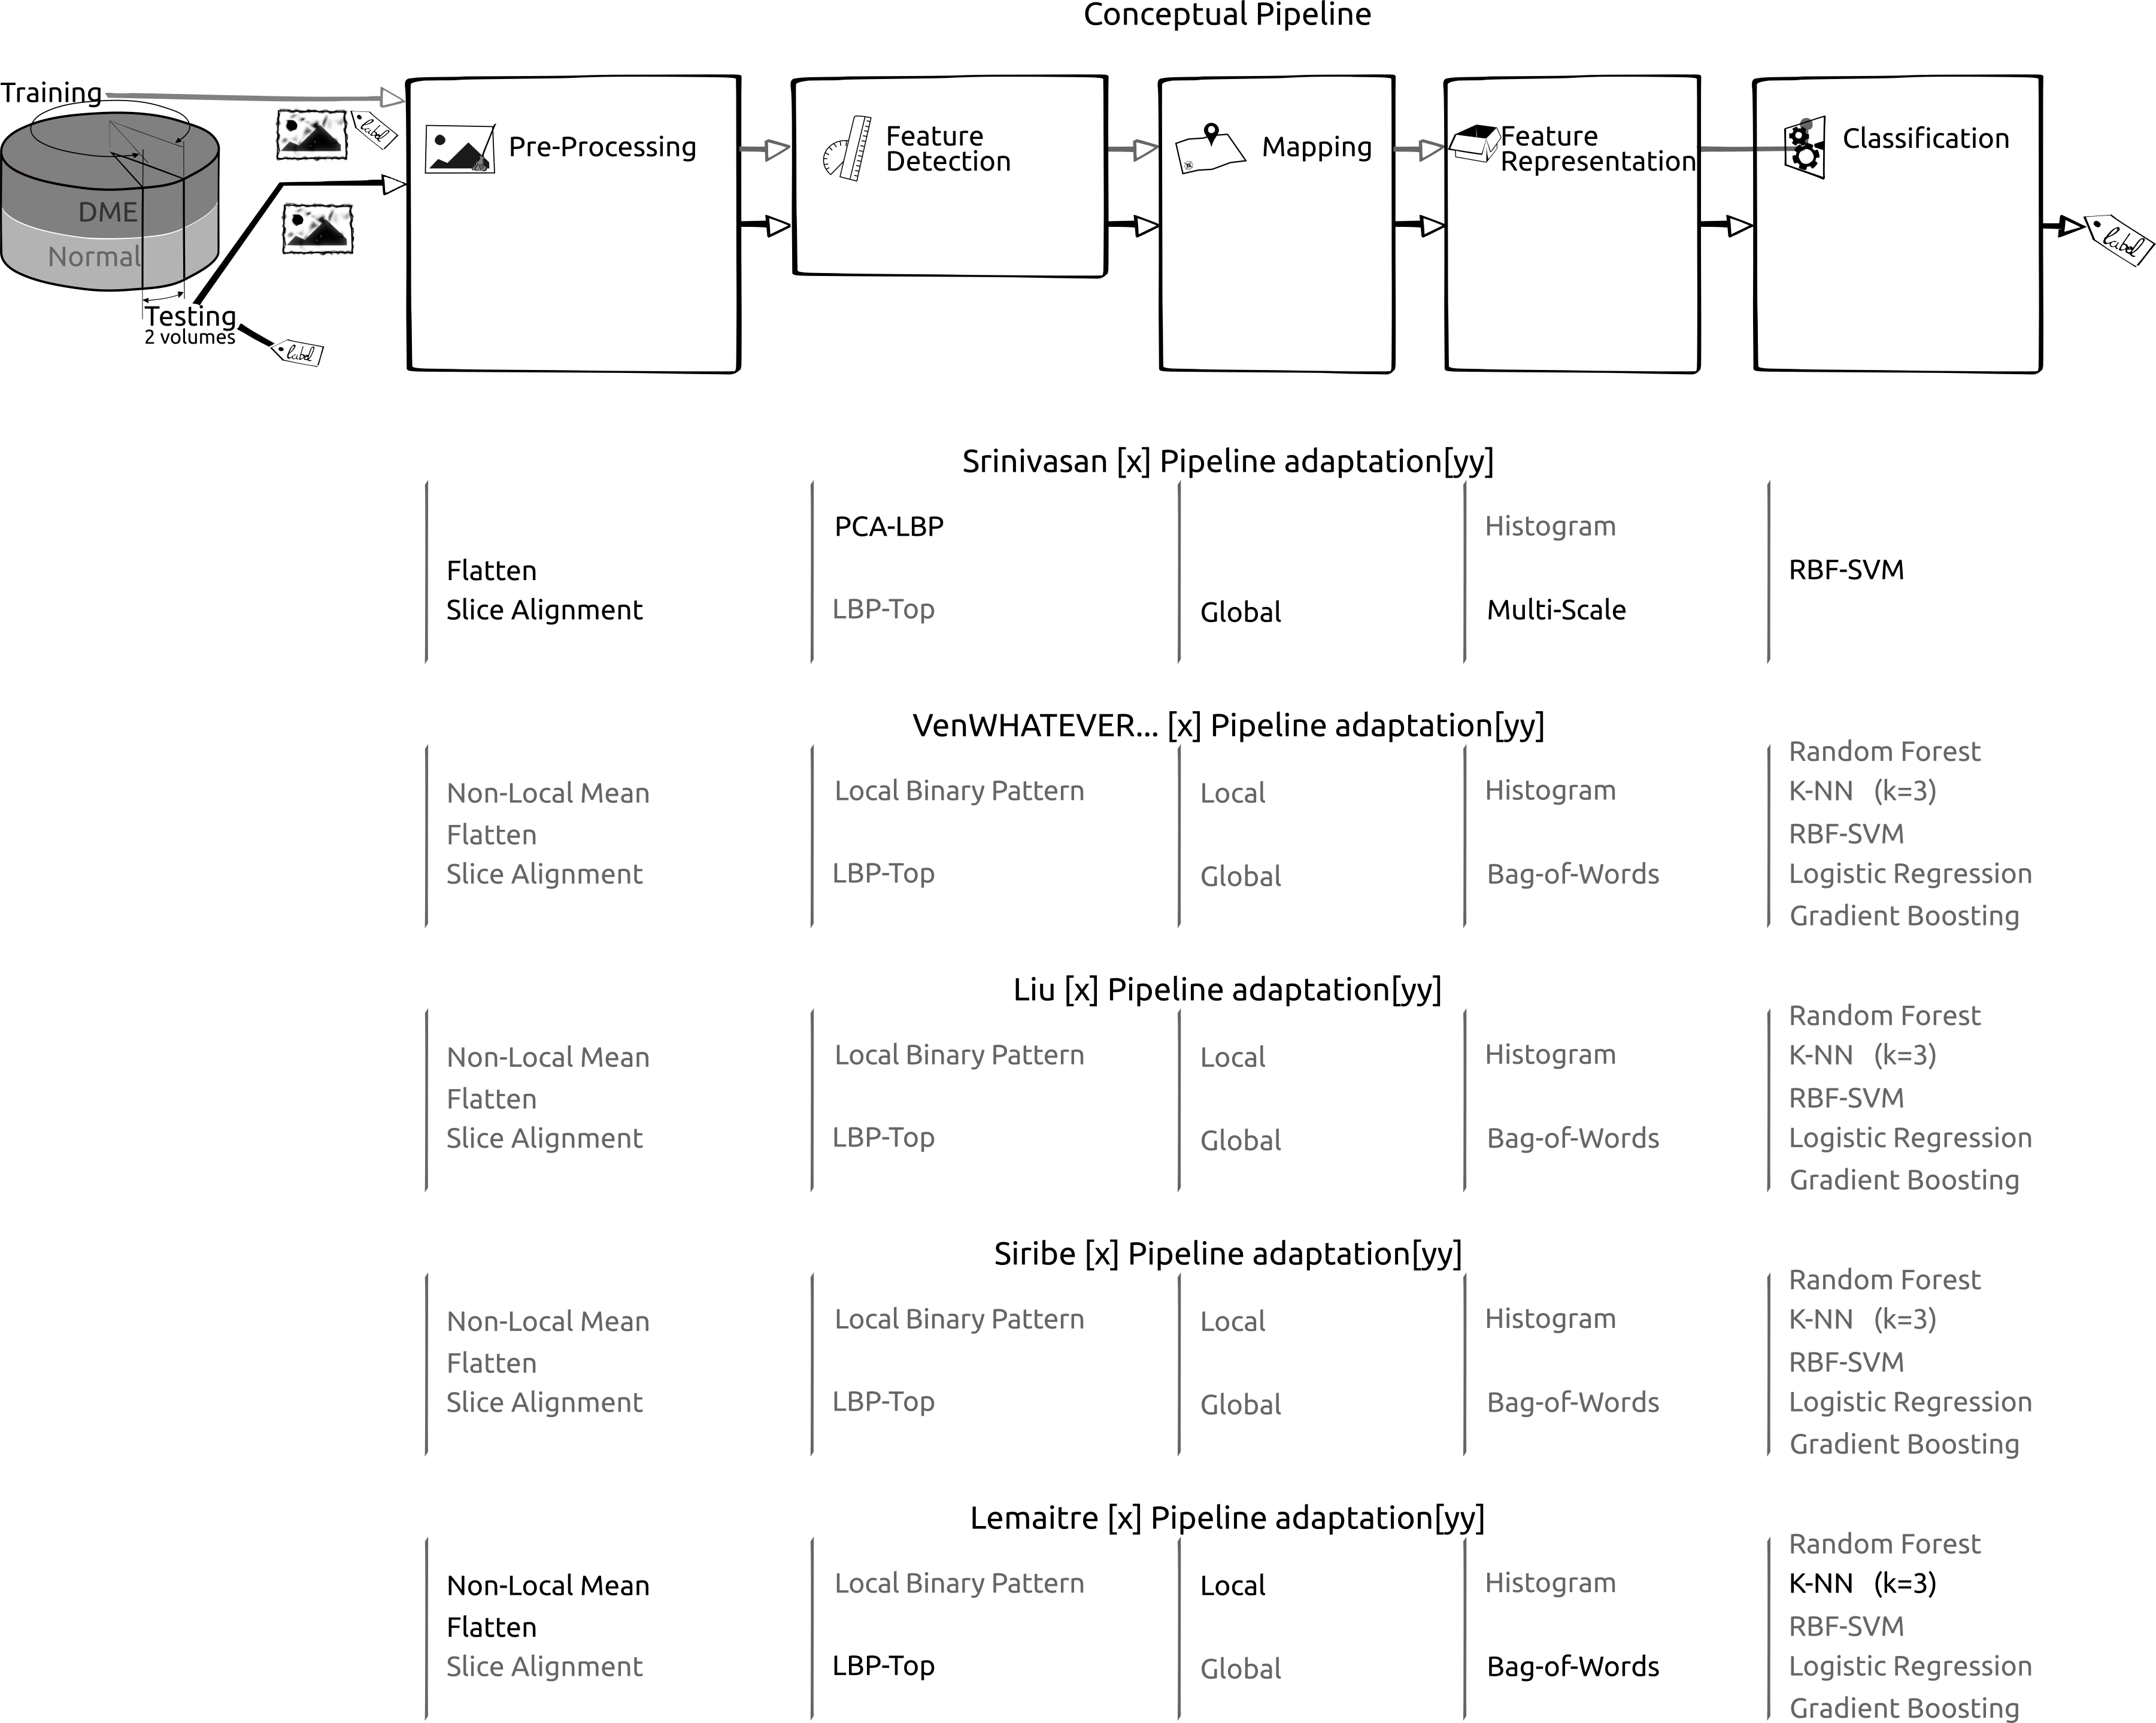
\includegraphics[width=1\linewidth]{ml}}
    \caption{Experimental Setup}
  \label{fig:ML-scheme}
\end{figure*}

\begin{table}
  \caption{Correspondence between the most relevant methodologies reviewed in Sect.\,\ref{sec:review} and the proposed experimental framework.}
\resizebox{1\linewidth}{!}{
\footnotesize{
\begin{tabular}{l c	c c c c }
\toprule
\multicolumn{1}{c}{Ref} & Pre-processing & Features &  Mapping &  Representation & Classification\\
    &  &  &  &  & \\
\midrule
	&  &  &  &  & \\
%Venhuizen\,\textit{et al.}~
Venhuizen \textit{et al.}~\cite{Venhuizen2015,venhuizen2015feb-repoICPR} &  & Texton & Local   &\gls{bow}, \gls{pca}  & \gls{rf} \\
	&  &  &  &  & \\
%Srinivansan\,\textit{et al.}~
\multirow{3}{*}{Srinivasan \textit{et al.}~\cite{Srinivasan2014, srinivasan2014oct-repoICPR}} & De-noise & \multirow{3}{*}{\gls{hog}} & \multirow{3}{*}{Global} & &  \multirow{3}{*}{linear-\gls{svm}} \\
 & Flatten & & & & \\
 & Cropped & & & & \\
	&  &  &  &  & \\
%Lema\^itre\,\textit{et al.}~
Lemaitre \textit{et al.}~\cite{Lemaintre2015miccaiOCT, lemaitre2015apr-repoICPR} & De-noised & \gls{lbp} & Local &  \gls{pca}, &  \gls{rf} \\
& & \gls{lbptop} & Global & \gls{bow}, Histogram & \\ 
	&  &  &  &  & \\

Alsaih \textit{et al.}~\cite{Alsaih2016apr-repoICPR} & ********* & \gls{lbp} & ***** &  \gls{pca}, &  \gls{rf} \\
& & \gls{lbptop} & ****** & \gls{bow}, ********* & \\ 
	&  &  &  &  & \\

%Liu\,\textit{et al.}~
% \multirow{2}{*}{Liu \textit{et al.}~\cite{Liu2011}} & Flatten & \multirow{2}{*}{Edge, \gls{lbp}} & \multirow{2}{*}{Local} & \multirow{2}{*}{\gls{pca}}& \multirow{2}{*}{\gls{rbf}-\gls{svm}} \\
% & Aligned & & & & \\
% 	&  &  &  &  & \\

%\midrule
\hdashline \noalign{\vskip 3pt}
\multirow{3}{*}{Sankar \textit{et al.}~\cite{sankar2016classification, sankar2015feb-repoICPR}} & De-noised & Pixel & \multirow{3}{*}{Global} & \multirow{3}{*	}{\gls{pca}} & Mahalanobis \\
 & Flatten &-intensities & & & -distance\\
 & Cropped & & & & to \gls{gmm}\\ 
\bottomrule
\end{tabular}}
}
\label{tab:survey-tab}
\end{table}

%\begin{table*}
%\caption{Summary of the state-of-the-art methods.}
%\resizebox{1.05\linewidth}{!}{
%\scriptsize{
%\begin{tabular}{l ccc c cccc	c c c c	c c}
%\toprule
%Ref & \multicolumn{3}{c}{Diseases} & Data  & \multicolumn{4}{c}{Pre-processing} & Features & Representation & Classifier & Evaluation & Results\\
%    &  &  &  & size &  &  &  &  &  &  &  & & &\\
%   \cmidrule(l){2-4}\cmidrule(l){6-9} 
%    & \gls{amd} & \gls{dme} & Normal  &           & De-noise & Flatten & Aligning & Cropping &   & &   &  &   \\
%\midrule
%& & & & & & & & & & & & & &  \\
%%Srinivansan\,\textit{et al.}~
%\cite{Srinivasan2014} & $\checkmark$ & $\checkmark$ & $\checkmark$ &  45 & $\checkmark$ & $\checkmark$ &  & $\checkmark$ & \gls{hog} &  & linear-\gls{svm} & \gls{acc} & 86.7\%,100\%,100\%  \\
%& & & & & & & & & & & & &    \\
%%Venhuizen\,\textit{et al.}~
%\cite{Venhuizen2015} & $\checkmark$ &  & $\checkmark$ & 384 &  & & & &  Texton  &\gls{bow}, \gls{pca}  & \gls{rf} & \gls{auc} & 0.984 \\ 
%& & & & & & & & & & & & &   & \\
%%Liu\,\textit{et al.}~
%\cite{Liu2011} & $\checkmark$ & $\checkmark$ & $\checkmark$  & 326 &  & $\checkmark$ & $\checkmark$ &  &  Edge, \gls{lbp} & \gls{pca}& \gls{svm}-\gls{rbf} &\gls{auc} & 0.93 \\
%& & & & & & & & & & & & & \\
%%Lema\^itre\,\textit{et al.}~
%\cite{Lemaintre2015miccaiOCT} &  & $\checkmark$ & $\checkmark$ & 62  & $\checkmark$ &  &  &  & \gls{lbp}-\gls{lbptop} & \gls{pca}, \gls{bow}, histogram&  \gls{rf} & \gls{se},\gls{sp} & 87.5\%, 75\%  \\
%& & & & & & & & & & & & &  \\
%\bottomrule
%\end{tabular}}}
%\label{tab:survey-tab}
%\end{table*}


\subsection{\deleted[id=sik]{method comments}}
\todo[inline]{here goes a description left to right of the modules, making remarks of the difference between the needs of each method.}
\added[id=old]{
First, the \gls{oct} volumes are pre-processed as presented in details in Sect.\,\ref{subsec:prepro}.
%Then toward a final descriptor \gls{lbp} and \gls{lbptop} features are extracted with different mapping strategy and represented using two approach.
Then, \gls{lbp} and \gls{lbptop} features are detected, mapped and represented as discussed in depth in Sect.\,\ref{subsec:feaext}, Sect.\,\ref{subsec:mapping}, and Sect.\,\ref{subsec:fearep}, respectively.
%{\color{red}The feature extraction, mapping, and representation are presented in depth in Sect.\,\ref{subsec:feaext}, Sect.\,\ref{subsec:mapping}, and Sect.\,\ref{subsec:fearep}, respectively. CHECK THE SECTION ORDERING}
Finally, the classification step is presented in Sect.\,\ref{subsec:cls}.
}

\deleted[id=sik]{The mapping in A is computed in this manner while in B this comes on the other side bla bla bla}


\subsection{Validation}\label{sec:exp:validation}
\added[id=old]{
All the experiments are evaluated in terms of \gls{se} and \gls{sp} using the \gls{lopocv} strategy, in line with \cite{Lemaintre2015miccaiOCT}.
\gls{se} and \gls{sp} are statistics driven from the confusion matrix (see Fig.\,\ref{fig:CM}) as stated in Eq.\,\eqref{eq:sesp}.
The \gls{se} evaluates the performance of the classifier with respect to the positive class, while the \gls{sp} evaluates its performance with respect to negative class.
}
\begin{align}
 \gls{se}  = \frac{TP}{TP+FN} \qquad \gls{sp} = \frac{TN}{TN+FP}
 \label{eq:sesp}
\end{align}
\added[id=old]{
The use of \gls{lopocv} implies that at each round, a pair \gls{dme}-normal volume is selected for testing while the remaining volumes are used for training.
Subsequently, no \gls{se} or \gls{sp} variance can be reported.
However, \gls{lopocv} strategy has been adopted despite this limitation due to the reduced size of the dataset.
}

\subsection{Management of data depending terms}
\deleted[id=sik]{
  Be aware that when computing the GMM~\cite{repo_des}, or the dictionary
  \cite{repo_lem}, only the training data for the current fold is used.
  Therefore such modules are recomputed at each fold.
}
\deleted[id=sik]{
  Other parameter tuning such the case of XXXX and YYYYY are also carried out using only ZZZZ
}
